\documentclass[openany, a4, 11pt]{book}

% Documentul va fi tradus in limba romana
\usepackage[romanian]{babel}

% Scriem cu diacritice... 
\usepackage[utf8x]{inputenc}

% Vom folosi si un appendix simplut
\usepackage[page]{appendix}

% Se importa si pachetul pentru URL-uri (acestea vor fi colorate cu albastru)
\usepackage{hyperref}
\usepackage[pdftex]{graphicx}    
\usepackage{subfig}
\usepackage{multicol}
\usepackage{color}
\usepackage{indentfirst}
\usepackage{pifont}
\usepackage[margin=2.8cm, vmargin={1.4in, 1.4in}]{geometry}
% \usepackage[bindingoffset=0.2in, left=1.0in, right=1.0in]{geometry}

% Pachetele necesare pentru crearea si afisarea formulelor matematice
\usepackage{mathtools}

% Folosim un pachet pentru antet si subsol
% Micsoreaza fontul in fancyhdr pentru a nu mai exista overlay-uri
\usepackage{fancyhdr, blindtext}
\newcommand{\changefont}{%
    \fontsize{9}{11}\selectfont
}
\fancyhf{}
\fancyhead[LE,RO]{\changefont \slshape \rightmark}
\fancyhead[RE,LO]{\changefont \slshape \leftmark}
\fancyfoot[C]{\changefont \thepage}
\pagestyle{fancy}

% Pachetele necesare pentru listarea de cod sursa
\usepackage{caption}
\usepackage{listings}
\usepackage{xcolor}

% Pachetele necesare pentru crearea unor casute cu diverse mesaje
\usepackage{styles/boxes}

\usepackage{array}
\usepackage{booktabs}
\usepackage{multirow}

% Pachete necesare pentru desenarea unor figuri pe ecranul utilizatorului
\usepackage{wrapfig}
\usepackage{graphicx}
\usepackage{subfig}

% Importam si pachetul necesar pentru QR code
\usepackage[]{qrcode}

\definecolor{gray}{RGB}{235,235,235}
\definecolor{codegreen}{rgb}{0,0.6,0}
\definecolor{codegray}{rgb}{0.5,0.5,0.5}
\definecolor{codepurple}{rgb}{0.58,0,0.82}
\definecolor{backcolour}{rgb}{0.95,0.95,0.92}

\renewcommand*\lstlistingname{Cod sursă}

% Numele paginii de Aneze din cuprins este redenumit
\renewcommand{\appendixtocname}{Anexă}

% Legaturile web vor fi colorate cu albastru
\newcommand{\myhref}[3][blue]{\href{#2}{\color{#1}{#3}}}%

% Alte modificari de configurare
\renewcommand{\headrulewidth}{1pt}
\renewcommand{\footrulewidth}{1pt}
\setlength{\headheight}{12pt}
\setcounter{secnumdepth}{6}
% Adancimea cuprinsului...
\setcounter{tocdepth}{3}
% Seteaza identarea unui paragraf
\setlength{\parindent}{1cm}

% Pentru cuprins se scoate culoarea si bordarea legaturilor
\hypersetup{urlbordercolor={1 1 1}, linkbordercolor={1 1 1}, citebordercolor={1 1 1}}

% De aici incepe documentul nostru...
\begin{document}

\newgeometry{margin=3cm}
\begin{titlepage}

% Titlul va aparea centrat
\begin{center}
 
\begin{figure}[htb]
\center{

\includegraphics[width=0.4 \textwidth]{images/logo.png}
}
\end{figure}
\noindent{\rule{8cm}{0.4pt}}\\[0.3cm]
\textsc{\Large Universitatea Politehnica București}\\[5.0cm]

{\Huge Politica de securitate}\\[0.4cm]
\textsc{\Large a platformei de forumuri\\ MyBB}\\[5.0cm]

% Informatii despre autor si despre indrumator
\begin{minipage}{0.5\textwidth}
\begin{flushleft}
\large{\textbf{Studenți}}\\
\large{Ionuț-Cătălin Barbu\\Mihai Surdeanu}
\end{flushleft}
\end{minipage}
~
\begin{minipage}{0.4\textwidth}
\begin{flushright}
\large{\textbf{Îndrumător}}\\
Omar-Salim Choudary\\
\end{flushright}
\end{minipage}\\[3.0cm]

% Alte informatii aditionale?
\noindent{\rule{8cm}{0.4pt}}\\[0.3cm] 
{\large ianuarie 2016}\\[1cm] 

\end{center}

% Trecem la urmatoarea pagina...
\end{titlepage}
\restoregeometry

% Setarile necesare pentru a include cod sursa in cadrul acestei documentatii
\lstdefinestyle{customc}{
    backgroundcolor=\color{backcolour},   
    commentstyle=\color{codegray},
    keywordstyle=\color{green!40!black},
    stringstyle=\color{codepurple},
    basicstyle=\footnotesize,
    numberstyle=\tiny\color{codegray},
    identifierstyle=\color{blue},
    belowcaptionskip=1\baselineskip,
    breaklines=true,
    language=C,
    showstringspaces=false,
    captionpos=b,                    
    keepspaces=true,                 
    numbers=left,                    
    numbersep=5pt,                  
    showspaces=false,                
    showstringspaces=false,
    showtabs=false,                  
    tabsize=2
}

% Sectiunea "Abstract"
\newgeometry{margin=5cm}
\thispagestyle{empty}
\begin{multicols}{2}
[
\section*{Cuvânt înainte,}
]
\footnotesize {
În ziua de astăzi, internetul este bazat pe o structură avansată hardware și software ce se află într-o continuă dezvoltarea. Domeniul IT, în general, nu a fost la saturație și nici nu pare să ajungă în următorii zeci de ani. Din ce în ce mai multe dispozitive sunt interconectate, din ce în ce mai multe lucruri sunt realizate cu ajutorul lui. Pe zi ce trece, informația care este pusă la dispoziție crește din punct de vedere al cantității, fiind disponibilă utilizatorului prin intermediul site-urilor web. \textbf{Forumul} reprezintă un mediu virtual, prin care utilizatorii pot discuta diverse lucruri, acoperind o plajă foarte mare de subiecte din diverse domenii.

Din păcate, o dată cu trecerea timpului, forumurile au început să nu mai fie la modă. Au avut un apogeu undeva pe la începutul anilor 2010.
Tendința din ultimii doi ani, a fost o scădere drastică a numărului de noi forumuri înființate, probabil și pe fondul apariției a tot mai multor bloguri și rețele sociale. Nu avem de-a face decât cu o consecință a foaptului că servicile de găzduire web au devenit din ce în ce mai accesibile, iar cunoștiințele necesare administrării unui forum regăsindu-se foarte ușor prin intermediul unor articole / tutoriale.

Asta nu înseamnă că forumurile au dispărut. Cele deja existente și care activează pe o anumită nișă, sunt încă la mare căutare. Ele concentrează o cantitate destul de mare de informație sensibilă, într-adevăr nu la fel de sensibilă ca cea expusă de o bancă sau un magazin virtual, dar care poate fi folosită în mod indirect pentru obținerea altor informații. De ceea partea de securitate reprezintă încă o provocare.
}
\end{multicols}

\vspace{1cm}

\begin{center}
    \qrcode[height=3cm]{http://www.mybb.com}
\end{center}

\restoregeometry

% Se afiseaza si un cuprins avansat
\tableofcontents

% Pagina cu lista de figuri
\renewcommand\listfigurename{Listă de figuri}
\listoffigures

% Sectiunea de introducere
\chapter{Introducere}
TODO

\subsection{TODO}
TODO


% Prezentarea detaliata a politicii curente
\chapter{Politica de securitate}

Platforma \textit{MyBB} pune un accent foarte important pe securitate. Conform site-ului oficial, securitatea este cea mai mare proprietate. Cu toate acestea, dezvoltatorii sunt conștienți că orice e făcut de om este pasibil să conțină buguri / erori, de aceea au încercat să atragă utilizatorii să contribuie și ei la această latură. Au încercat să introducă un sistem de reward-uri, care la companiile mari se traduce în oferirea unei sume de bani în funcție de vulnerabilitatea submisă. Aici din păcate avem de-a face cu un proiect open source, un proiect în spate căruia nu există o companie, există doar ideea de voluntariat. Nu negăm că există o serie de oameni dispuși să doneze pentru o cauză, dar de multe ori aceste donații se reinvestesc în infrastructură în vederea menținerii proiectului online. Ca să nu o mai lungim foarte mult, cei care descoperă vulnerabilități și le raportează echipei MyBB vor fi trecuți pe o pagină onorifică a site-ului oficial - numită \textit{Security Hall of Fame}.

Este printre puținele platforme open source căreia i s-a făcut și un audit de securitate. Auditul a fost făcut în anul 2008, de către GulfTech. În urma acestui audit, s-a identificat câteva probleme și s-a putut trage concluzia că MyBB prezintă un low-risk record în ceea ce privește nivelul de securitate. Nici din punct de vedere istoric nu au fost găsite foarte multe high-risk vulnerabilități. De multe ori e important să înveți din greșeli, din problemele apărute de-a lungul timpului.

Tot de pe site-ul oficial - \textit{http://mybb.com}, se pot regăsi și câteva instrucțiuni pe care echipa MyBB le pune la dispoziție utilizatorilor. Până la urmă degeaba ai un sistem foarte sigur, dacă cei care îl administrează nu o fac corect. De aceea, trebuie cumva educați administratorii pentru a preîntâmpina diverse neplăceri mai târziu. Nu putem să le numim reguli. Ar fi doar niște recomandări. Le vom prezenta succint în paragrafele următoare.

\section{Actualizări periodice}

Utilizatorul trebuie să se asigure că are întotdeauna cea mai nouă versiune a platformei. Echipa MyBB este foarte proactivă și fixează o vulnerabilitate high-risk în cel mult 48 de ore. Numărul de actualizări pe an nu este foarte mare, o actualizare apare la un interval de 2-3 luni. Ce ar trebui să reținem aici? Faptul că actualizările sunt determinate în principiu de fixarea unei vulnerabilități importante sau introducea unui set major de feature-uri.

\section{Ascunderea versiunii platformei}

În ceea ce privește afișsarea versiunii curente a platformei, MyBB adoptă o politică diferită față de majoritatea competitorilor, în sensul în care în mod implicit versiunea platformei nu este afișată în subsol, alături de copyright. Cu cât cunoști mai puține lucruri despre un sistem, cu atât este mai greu să îl spargi. Asta nu înseamnă că administratorul nu are posibilitatea de a dezactiva acest comportament din panoul de administrare, dacă asta e ceea ce își dorește.

\section{Panoul de administrare}

Ca și majoritatea celorlalte platforme web, un forum oferă \textit{două interfețe}, o interfață de tip \textit{front-end} - forumul propriu-zis - unde predomină operațiunile de citire și un altă interfață de tipul \textit{back-end} - panoul de administrare - unde predomină operațiile de scriere. Din motive evidente, cea mai riscantă zonă din punct de vedere a securității o reprezintă cea de-a doua și anume panoul de administrare. O dată ce un utilizator a obținut acces la această zonă, el are control asupra întregului forum.

În acest sens, echipa MyBB ține să sublinieze faptul că panoul de administrare este doar pentru administratori. Celelalte grupuri de utilizatori nu au acces implicit la această zonă. Contează și numărul de administratori din sistem: \textbf{"More Admins = Less Security"}

Panoul de administrare trebuie ascuns, trebuie ținut la distanță de ceilalți utilizatori care nu au privilegii de administratori. De aceea ar fi bine să fie redenumit directorul în care se regăsesc sursele PHP pentru această zonă, din \textit{admin} în ceva mult mai bizar, folosind un string random. În acest caz, cel care pregătește un atac, sau are intenții mai puțin bune, trebuie să petreacă mai mult timp în descoperirea căii către panoul de administrare. Se poate merge și mai departe prin securizarea panoului de administrare folosind \textit{HTTP Basic Auth} cu o parolă adițională.

\subsection{Cod PIN}

\begin{wrapfigure}{r}{0.5\textwidth}
    \vspace{-60pt}
    \center{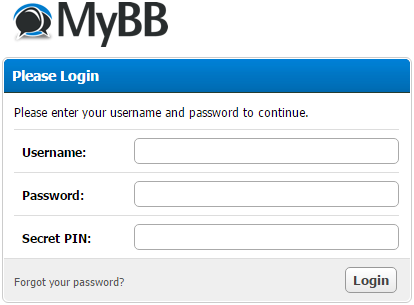
\includegraphics[width=0.5 \textwidth]{images/login.png}}
    \vspace{-20pt}
    \caption{\label{fig:Policy-AdminLogin} Autentificarea în AdminCP}
    \vspace{-10pt}
\end{wrapfigure}

Începând cu versiunea 1.8, în cadrul platformei s-a mai introdus un feature prin intermediul căruia se poate seta un cod PIN asupra panoului de administrare. Codul este format din 4 cifre și este static, putând fi modificat manual de administrator doar folosind accesul fizic la fișierele de configurare. Chiar dacă aduce un plus de securitate, prin cererea unor informații adiționale la autentificare, un dezavantaj ar fi faptul că acest cod nu se modifică automat după o perioadă de timp, modificările sale rămânând la latitudinea administratorului. În figura \ref{fig:Policy-AdminLogin} se poate observa existența acestui secret PIN.

\subsection{Backup-uri regulate}

Tot din panoul de administrare se poate configurare realizarea de backup-uri automate ale bazei de date la intervale periodice de timp. Procesul de backup este automatizat complet, arhiva rezultată putând fi păstrată pe server sau trimisă pe email, în cazul în care dimensiunea arhivei nu depășește 10 MB. Nu este necesar să facem un backup și la fișierele platformei pentru că acestea în mod normal ar trebui să fie recuperate ușor, fiind identice cu cele de pe site-ul oficial.

\section{Sistemul de modificări}

Platformei MyBB i se poate extinde funcționalitatea prin adăugarea unor modificări. Aceste modificări se numesc în termeni populari plugins. Sistemul de modificări funcționează prin intermediul interceptării unor evenimente ce au loc înainte sau după anumite acțiuni importante. Fiecare extensie, înregistrează la un dispatcher acțiunile pe care dorește să fie rulate atunci când un eveniment are loc. Așa după cum vă puteți da seama, fișierele de core nu sunt modificate sub nicio formă la instalarea unei noi modificări.

Comportamentul este puțin diferit față de ceea ce regăsim spre exemplu la platforma \textit{phpBB}, în care instalarea unei modificări presupune modificare unui sau mai multor fișiere din core. În cazul nostru, avantajul este reprezentat de faptul că fișierele de core rămân intacte, dezavantajul fiind introducerea unui overhead prin faptul că există un număr mai mare de apeluri de funcții. Se poate spune că securitatea este sporită în detrimentul performanței!

\newboxedtheorem[boxcolor=none, background=blue!5, titlebackground=blue!20, titleboxcolor = none]{theo}{Studiu de caz}{anything}
\begin{theo}[Număr de modificări utilizate]
Cu cât numărul de modificări instalate pe o platformă MyBB este mai mic cu atât riscurile în apariția unor vulnerabilități este mai mic. Momentan nu există o metodă prin care modificările realizate de către alți developeri să fie testate riguros, motiv pentru care acestea pot mai avea scăpări, introducând diverse probleme de securitate.\\
\textbf{Concluzie:} La ora actuală cele mai mari probleme de securitate au fost cauzate de tot felul de modificări.
\end{theo}

O să vedem un pic mai târziu ce face comunitatea oficială pentru a reduce numărul de modificări cu probleme de securitate.

\section{Controlul accesului în sistem}

TODO - Aici trebuie să vorbim despre grupurile de utilizatori.

\section{Filtrarea informației}

TODO - Aici trebuie să vorbim despre cum este tratată informația din mediul extern. ce se face pentru a evita injectarea de cod?

\section{Sesiuni și parole}

TODO

\section{Interacțiunea cu comunitatea oficială - \textit{MyBB.com}}

TODO

% Posibile imbunatatiri ce pot fi realizate
\chapter{Îmbunătățiri}

O politică de securtitate nu poate proteja niciodată utilizatorii și administratorii de posibile breșe de securitate; asftel se duduce din acest lucru ca unei politici de securitate i se pot aduce oricând îmbunătățiri. Un alt aspect din care este privită o politică de securitate este modul în care vrem să protejeze aplicația noastră: putem dori sa aibă mai puține restricții, dar să ofere mult mai multe facilități care să fie mult mai ușor accesibile sau putem avea o securitate sporită prin care să obligăm utilizatorii si administratorii să realizeze mult mai multe taskuri din punct de vedere al securității și sa aibă mai acces restricționat acolo unde nu este necesar să aibă.

\section{Codul Pin}

O posibilă îmbunătățire adusă în privința panoului de administrare se referă la codul pin. Cu privire la acest cod pin nu există o politică prin care să se reglementeze o anumiă perioada la care acesta să fie schimbat și de asemenea nu există un sistem de notificare pentru schimbarea acestuia. Astfel că o îmbunătățire consta în adăugarea opțiunii de a fi schimbat cel puțin o dată într-o perioadă de minim 1 lună și maxim 3 luni. Un ajutor cu privire la acest aspect ar fi ca înainte cu 10 zile ca pinul să expire administratorului să îi fie trimis un email zilnic prin care să i se reamintească faptul că trebuie să schimbe acest pin. O verificare suplimentară ar fi ca un administrator să nu poată seta acelși pin decât după ce a avut setate alte 5 pinuri diferite. Modul de răspândire al pinului după o schimbare să se realizeze prin email către utilizatorii care au acces la modulele protejate cu ajutorul codului pin. 

Tot referitor la codul pin, atunci când acesta este introdus greșit de cinci ori și parola și username-ul sunt corecte userului să îi fie blocat accesul la panoul de administrare și să ii fie trimis un email de informare administratorului că cineva a încercat să introducă pinul de mai multe ori. Deblocarea accesului utilizatorului la consola de administrare să fie realizată manual de către administrator dupa confirmarea că însăși utilizatorul a introdus codul pin greșit. 

\section{Verificare bazată pe IP}

O verificare importantă cu referire la sistemul de autentificare se referă la faptul că nu poți din punct de vedere fizic acum să te loghezi din România, iar peste două ore să încerci să te loghezi din America, fiind aproape imposibil să ajungi dintr-un loc în altul. O chestie utilă ar fi ca la fiecare autentificare să se facă o verificare de IP pentru a se descoperi zona din care se încearcă logarea în sistem. În caz că zone nu corespunde cu zonele din care s-au realizat ultimele autenficări atunci userul sa fie blocat, iar deblocarea din această stare să se facă printr-un email de confirmare sau prin răaspund la întrebări de securitate.

Un caz în care verificarea pe bază de IP nu este chiar utilă este atunci când încerci să te autentifici dintr-un loc care are drept gateway un server din altă țară, caz în care IP este văzaut ca neaparținînd cu cele uzuale.

\section{Întrebări de verificare}

Schimbarea parolei se poate realiza în acest moment din cont atunci când ești logat cerându-se să se introducă și parola anterioară. O altă metodă pentru schimbarea parolei este prin accesarea featurelui de uitare parolă prin care se cere adresa de email cu care s-a făcut înregistrarea în sistem pentru a putea fi trimisă o nouă parolă utilizatorului. Pentru îmbunătățirea acestui modul ar fi utilă o metodă în plus de verificare și anume verificare prin întrebări de securitate. Astfel atunci cand își crează contul un utilizator să fie nevoit să își seteze două întrebări de securitate la care să știe doar el răspunsul. Acestea ar trebuie să poate fi editate și după crearea contului.

\section{Număr de autentificări greșite}

Când vine vorba de autentificare un utilizator poate greși din neatenție parola sau numele de utilizator de două trei ori. Când se întâmplă lucrul acesta utilizatorul trebuie anunțat cumva și asta s-ar putea realiza prin introducerea unui cod capcha care ar trebui introdus începând cu a cincea încercare de autentificare greșită. Modalitatea în care se depisteaa când un utilizator încearca în mod eronat să se autentifice ar trebui de altfel îmbunătățită. Astfel nu ar trebui salvate în cookieuri numărul de autentificări încercate, ci acestea să se salveze în cadrul forum-ului. Astfel se pot evita cazurile în care utilizatorul șterge cookieurile și astfel face bypass la acest nivel de securitate sau în cazurile cănd browserele sunt setate să nu salveze cookier-uri.

\section{HTML code}

În acest moment inserarea de cod HTML poate fi activată sau dezactivată de către un administrator. Introducerea de cod HTML poate reprezenta o breșă de securitate, iar din această cauză ar trebui limitată activarea/dezactivarea acestei opțiuni: activarea sau dezactivea ei să fie controlată doar de super administrator,astfel respectându-se ideea de cu cât mai puțină lume are acces cu atât mai sigură este.

\section{Valabilitate sesiune}

În ceea ce privește valabilitatea sesiunii unui utilizator ce este administrator și are drept de acces la panoul de control aceasta ar trebui să aibă o limitare. Astfel atunci când un utilizator iese din zona panoului de administrare sesiunea ar trebui să expire, iar la o eventuală revenire să trebuiască să reintroducă datele de autentificare chiar dacă operație de delogare nu s-a făcut explicit.

% Posibile imbunatatiri ce pot fi realizate
\chapter{Concluzii}
TODO

% Sectiunea de referinte va fi mereu pe o alta pagina
\newpage

% Avem si o scurta sectiune cu anexe.
\renewcommand{\appendixpagename}{Anexă}
\setcounter{figure}{0} 
\begin{appendices}

\end{appendices}

% Dezvoltarea unei aplicatii in CodeWarrior for MCU
% Redenumim anumite comenzi
\renewcommand*{\refname}{Referințe bibliografice}

% Referinte...
\begin{thebibliography}{00}
\bibitem{toDo} TODO
\end{thebibliography}

% Se adauga si pagina de bibliografie la cuprins
\addcontentsline{toc}{chapter}{Bibliografie}

% Sfarsitul documentului
\end{document}